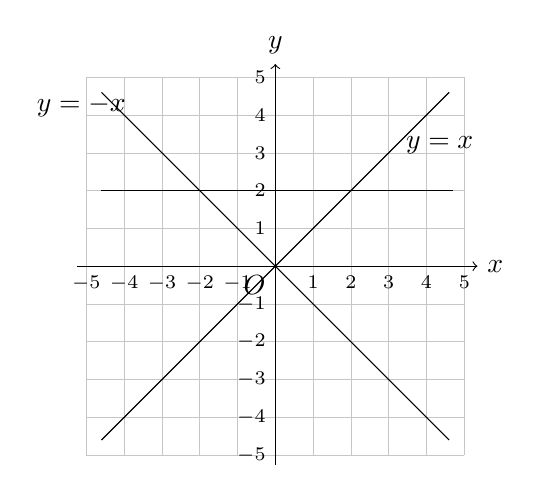
\begin{tikzpicture}[x=.48cm,y=.48cm,baseline=(current bounding box.center)]
  \draw[step=1,gray!45,very thin] (-5,-5) grid (5,5);
  \draw[->] (-5.25,0)--(5.35,0) node[right] {$x$}; \draw[->] (0,-5.25)--(0,5.35) node[above] {$y$};
  \draw (-4.6,2)--(4.7,2); \draw (-4.6,4.6)--(4.6,-4.6); \draw (-4.6,-4.6)--(4.6,4.6);
  \node[above left] at (-3.7,3.7) {$y=-x$}; \node[right] at (3.2,3.2) {$y=x$};
  \foreach \v in {-5,-4,-3,-2,-1,1,2,3,4,5} {\node[below] at (\v,0) {\scriptsize $\v$}; \node[left] at (0,\v) {\scriptsize $\v$};}
  \node[below left] at (0,0) {$O$};
\end{tikzpicture}
